\documentclass[
11pt, % The default document font size, options: 10pt, 11pt, 12pt
codirector, % Uncomment to add a codirector to the title page
]{charter} 




% El títulos de la memoria, se usa en la carátula y se puede usar el cualquier lugar del documento con el comando \ttitle
\titulo{Firmware de comunicaciones para un tren motor} 

% Nombre del posgrado, se usa en la carátula y se puede usar el cualquier lugar del documento con el comando \degreename
\posgrado{Carrera de Especialización en Sistemas Embebidos} 
%\posgrado{Carrera de Especialización en Internet de las Cosas} 
%\posgrado{Carrera de Especialización en Intelegencia Artificial}
%\posgrado{Maestría en Sistemas Embebidos} 
%\posgrado{Maestría en Internet de las cosas}

% Tu nombre, se puede usar el cualquier lugar del documento con el comando \authorname
\autor{Marcos Raul Dominguez Shocron} 

% El nombre del director y co-director, se puede usar el cualquier lugar del documento con el comando \supname y \cosupname y \pertesupname y \pertecosupname
\director{A definir}
\pertenenciaDirector{pertenencia} 
% FIXME:No IMPLEMENTADO EL CODIRECTOR ni su pertenencia
\codirector{John Doe} % para que aparezca en la portada se debe descomentar la opción codirector en el documentclass
\pertenenciaCoDirector{FIUBA}

% Nombre del cliente, quien va a aprobar los resultados del proyecto, se puede usar con el comando \clientename y \empclientename
\cliente{Guillermo Gebhart}
\empresaCliente{Voltu Motors}

% Nombre y pertenencia de los jurados, se pueden usar el cualquier lugar del documento con el comando \jurunoname, \jurdosname y \jurtresname y \perteunoname, \pertedosname y \pertetresname.
\juradoUno{Nombre y Apellido (1)}
\pertenenciaJurUno{pertenencia (1)} 
\juradoDos{Nombre y Apellido (2)}
\pertenenciaJurDos{pertenencia (2)}
\juradoTres{Nombre y Apellido (3)}
\pertenenciaJurTres{pertenencia (3)}
 
\fechaINICIO{08 de marzo de 2022}		%Fecha de inicio de la cursada de GdP \fechaInicioName
\fechaFINALPlan{19 de abril de 2022} 	%Fecha de final de cursada de GdP
\fechaFINALTrabajo{a definir}	%Fecha de defensa pública del trabajo final


\begin{document}

\maketitle
\thispagestyle{empty}
\pagebreak


\thispagestyle{empty}
{\setlength{\parskip}{0pt}
	\tableofcontents{}
}
\pagebreak


\section*{Registros de cambio}
\label{sec:registro}


\begin{table}[ht]
	\label{tab:registro}
	\centering
	\begin{tabularx}{\linewidth}{@{}|c|X|c|@{}}
		\hline
		\rowcolor[HTML]{C0C0C0}
		Revisión & \multicolumn{1}{c|}{\cellcolor[HTML]{C0C0C0}Detalles de los cambios realizados} & Fecha            \\ \hline
		0        & Creación del documento                                                          & \fechaInicioName \\ \hline
		1        & Se completa hasta el punto 5 inclusive                                          & 13/03/2022       \\ \hline
		2        & Se completa hasta el punto 9 inclusive                                          & 20/03/2022       \\ \hline
		3        & Se completa hasta el punto 12 inclusive                                         & 29/03/2022       \\ \hline
		4        & Correcciones finales                                                            & 14/05/2022       \\ \hline

		%		  Se puede agregar algo más \newline
		%		  En distintas líneas \newline
		%		  Así                                                    & dd/mm/aaaa \\ \hline
		%3      & Se completa hasta el punto 11 inclusive                & dd/mm/aaaa \\ \hline
		%4      & Se completa el plan	                                 & dd/mm/aaaa \\ \hline
	\end{tabularx}
\end{table}

\pagebreak



\section*{Acta de constitución del proyecto}
\label{sec:acta}

\begin{flushright}
	Buenos Aires, \fechaInicioName
\end{flushright}

\vspace{2cm}

Por medio de la presente se acuerda con el Ing. \authorname\hspace{1px} que su Trabajo Final de la \degreename\hspace{1px} se titulará ``\ttitle'', consistirá implementar en el nuevo hardware de comunicaciones las funcionalidades existentes e incorporar funcionalidades de la placa de control, y tendrá un presupuesto preliminar estimado de 596 hs de trabajo y \$3.447.132, con fecha de inicio \fechaInicioName\hspace{1px} y fecha de presentación pública \fechaFinalName.

Se adjunta a esta acta la planificación inicial.

\vfill

% Esta parte se construye sola con la información que hayan cargado en el preámbulo del documento y no debe modificarla
\begin{table}[ht]
	\centering
	\begin{tabular}{ccc}
		\begin{tabular}[c]{@{}c@{}}Ariel Lutenberg \\ Director posgrado FIUBA\end{tabular} & \hspace{2cm} & \begin{tabular}[c]{@{}c@{}}\clientename \\ \empclientename \end{tabular} \vspace{2.5cm} \\
		\multicolumn{3}{c}{\begin{tabular}[c]{@{}c@{}} \supname \\ Director del Trabajo Final\end{tabular}} \vspace{2.5cm}                        \\
		%\begin{tabular}[c]{@{}c@{}}\jurunoname \\ Jurado del Trabajo Final\end{tabular}     &  & \begin{tabular}[c]{@{}c@{}}\jurdosname\\ Jurado del Trabajo Final\end{tabular}  \vspace{2.5cm}  \\
		%\multicolumn{3}{c}{\begin{tabular}[c]{@{}c@{}} \jurtresname\\ Jurado del Trabajo Final\end{tabular}} \vspace{.5cm}                                                                     
	\end{tabular}
\end{table}




\section{1. Descripción técnica-conceptual del proyecto a realizar}
\label{sec:descripcion}


Un Power Train o Tren Motor es el sistema encargado de impulsar los vehículos eléctricos. Estos convierten la energía eléctrica almacenada en baterías a motriz alimentando un motor eléctrico.

El tren motor es uno de los dos productos principales que desarrolla y comercializa la empresa Voltu Motors. Este Tren Motor puede adaptarse a diferentes tipos de vehículos, actualmente se han instalado en motos, cuatriciclos, colectivos y camiones.

El dispositivo consta de un pack de baterías, una unidad de control, el motor. La unidad de control de Voltu Motors utiliza dos placas microcontroladas para resolver el hardware.
La primera de ellas es un DSP que realiza el control para mover el motor y cargar las baterías . La segunda es la placa de comunicaciones que cumple la función de interactuar con el exterior de la unidad de control.

El usuario del vehículo puede controlar el Tren Motor mediante una interfaz gráfica, la cual se encuentra en el tablero del vehículo. Este tablero es una tablet que se comunica con la unidad de control mediante protocolo USB.

La placa de comunicaciones posee:

\begin{itemize}
	\item Entradas y salidas digitales para el manejo de periféricos como luces, ventiladores, etc.
	\item Interfaz USB para comunicarse con la tablet del usuario.
	\item Interfaz UART para comunicarse con la placa de control, una con fines de \textit{debug} y otra para comunicarse con el BMS (\textit{Battery Management System}).
	\item Interfaz para gestionar el conexionado de un EVSE (\textit{Electric Vehicle Supply Equipment}).
\end{itemize}

Las características listadas anteriormente convierten a la placa de comunicaciones en la encargada de gestionar el estado de la unidad de control. Esta utiliza la información que recibe de todas sus interfaces para la toma de decisiones.

Actualmente, existe una versión funcional con un hardware distinto en donde la placa de control gestiona gran parte de las tareas que se proponen para la nueva placa de comunicaciones.

La nueva implementación permitirá reducir las tareas del DSP a los algoritmos de control del motor y la carga, y mejora así la seguridad del sistema. Además, esta configuración incorpora nuevas características, como el manejo de distintos tipos de EVSE y la posibilidad de definir fuera de tiempo de compilación características del tren motor que se adapten a distintos tipos de vehículos.

%\vspace{25px}


En la Figura \ref{fig:diagBloques} se presenta el diagrama en bloques del sistema. Se puede observar como la placa de comunicaciones interactúa con la Tablet, el DSP y el BMS, mientras que la placa de control se encarga de controlar el flujo de energía para la carga de la batería o marcha del motor. Adicionalmente, la placa de comunicaciones gestiona las entradas y salidas con los periféricos del vehículo.

Debido a que la nueva versión del tren motor está planificada con este hardware, el desarrollo de este proyecto es fundamental para su lanzamiento.

\begin{figure}[htpb]
	\centering
	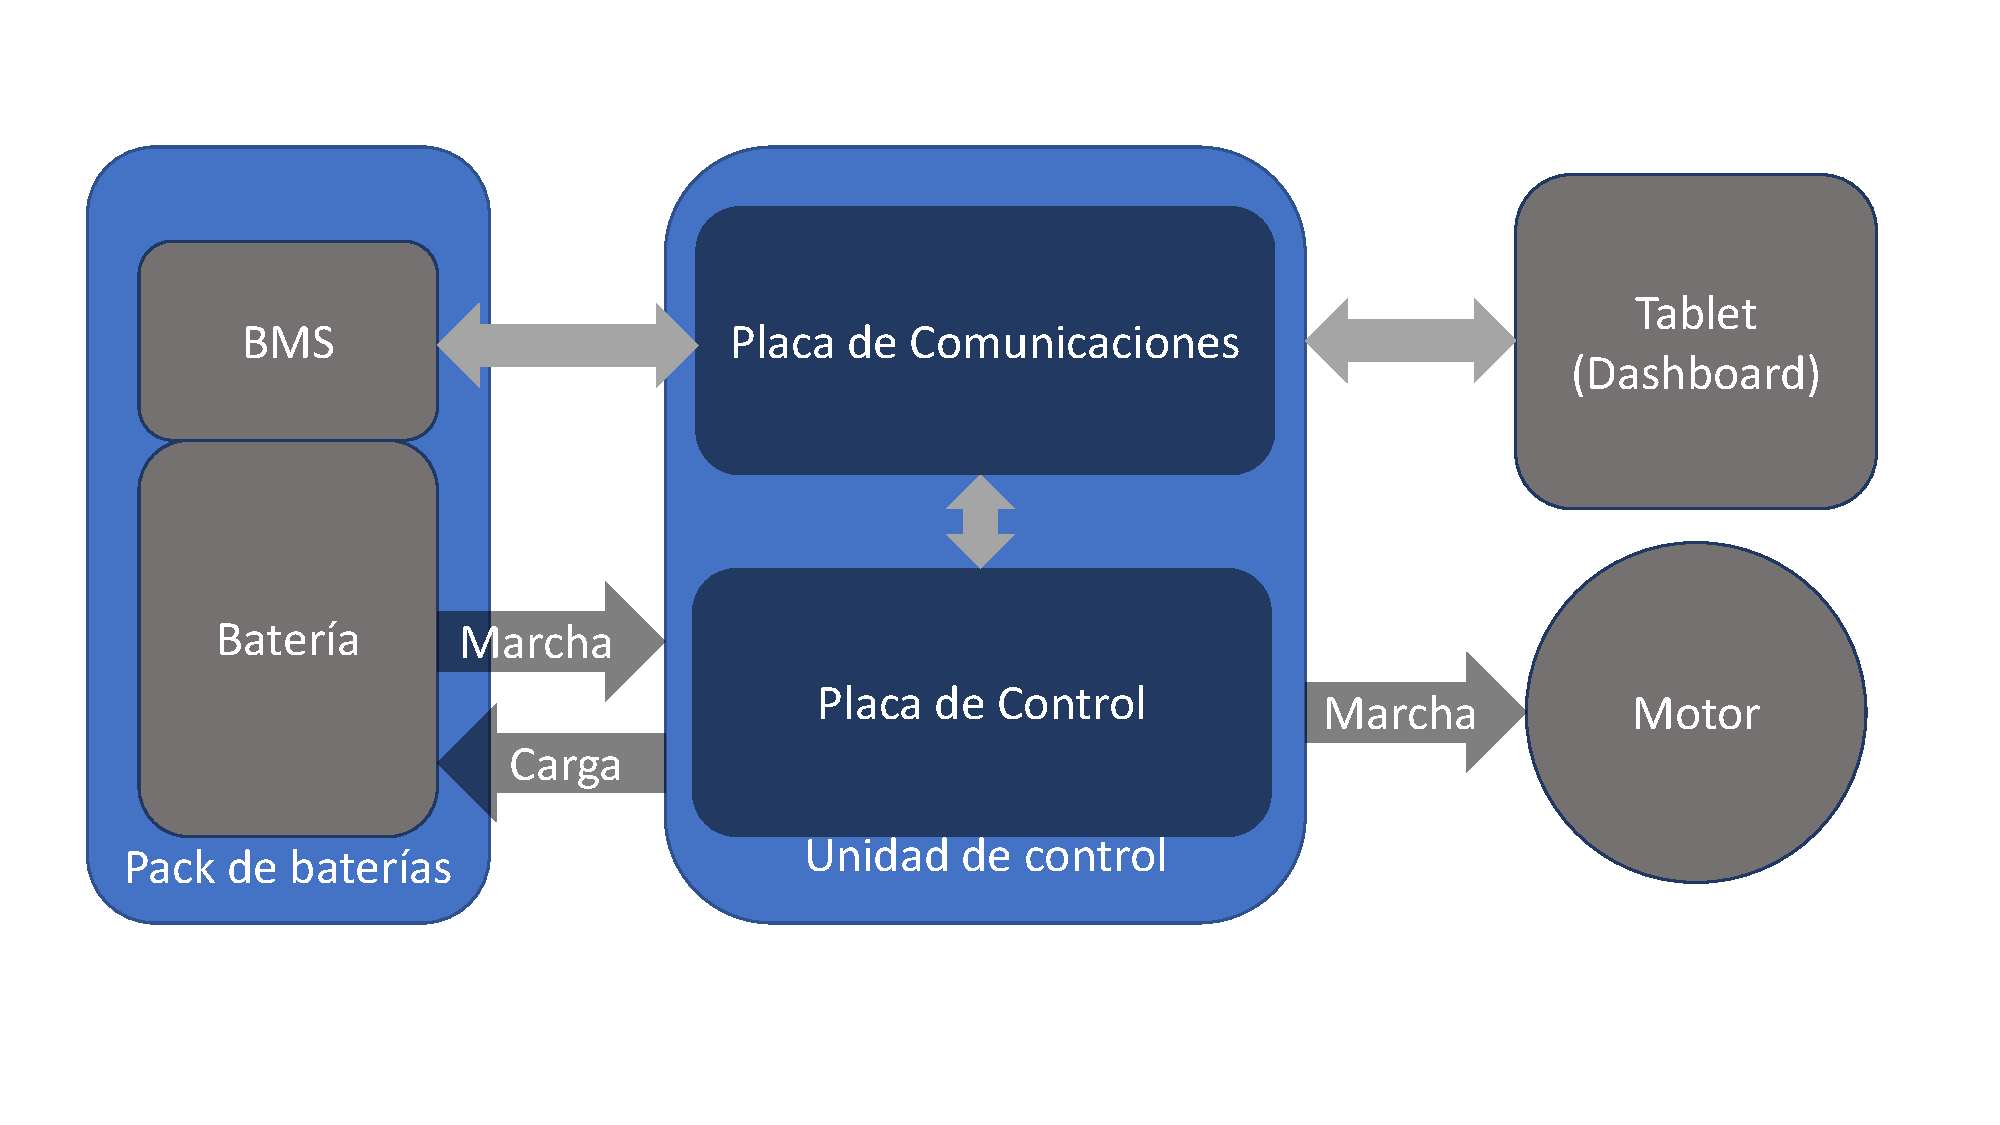
\includegraphics[width=.9\textwidth]{./Figuras/EsquematicoPT.pdf}
	\caption{Diagrama en bloques del sistema}
	\label{fig:diagBloques}
\end{figure}

\vspace{25px}

\section{2. Identificación y análisis de los interesados}
\label{sec:interesados}

\begin{table}[ht]
	%\caption{Identificación de los interesados}
	%\label{tab:interesados}
	\begin{tabularx}{\linewidth}{@{}|l|X|X|l|@{}}
		\hline
		\rowcolor[HTML]{C0C0C0}
		Rol           & Nombre y Apellido & Organización    & Puesto                      \\ \hline
		Auspiciante   & \clientename      & \empclientename & CEO y Fundador              \\ \hline
		Cliente       & \clientename      & \empclientename & CEO y Fundador              \\ \hline
		Impulsor      & Luciano Vittori   & \empclientename & Lider de Control y Firmware \\ \hline
		Responsable   & \authorname       & FIUBA           & Alumno                      \\ \hline
		Orientador    & \supname          & \pertesupname   & Director Trabajo final      \\ \hline
		Usuario final & Gonzalo Cuenca    & \empclientename & Testing y Calidad           \\ \hline
	\end{tabularx}
\end{table}





\section{3. Propósito del proyecto}
\label{sec:proposito}

El propósito de este proyecto es desarrollar el firmware de la nueva placa de comunicaciones. Este firmware debe cubrir las características de la versión anterior y además contemplar el manejo del BMS, EVSE y periféricos.
La nueva versión también será la encargada de realizar el control de temperatura del sistema.

\section{4. Alcance del proyecto}
\label{sec:alcance}

En el presente proyecto se diseñará, desarrollará e implementará el firmware de la placa de comunicaciones hasta que sea funcional para un vehículo que utilice una sola unidad de tren motor.
Esto incluye la implementación de las siguientes características:
\begin{itemize}
	\item Manejo de entradas y salidas digitales.
	\item Comunicación USB con el protocolo actual para la comunicación con la Tablet.
	\item Comunicación con placa de control, transmisión de datos y recepción de datos.
	\item Gestión del estado del vehículo.
	\item Administración de la batería (definir cuando cargar y balancear las celdas).
	\item Control de temperatura del sistema.
\end{itemize}

Este proyecto no incluye el diseño del hardware debido a que ya está preestablecido. El montaje del sistema en un vehículo particular tampoco está dentro del alcance del proyecto.


\section{5. Supuestos del proyecto}
\label{sec:supuestos}

Para el desarrollo del presente proyecto se supone que:

\begin{itemize}
	\item Se dispone del hardware de la nueva placa de comunicaciones.
	\item Se dispone de un banco de pruebas con el sistema completo para realizar pruebas de inmunidad al ruido del firmware.
	\item Se dispone de un EVSE para las pruebas de carga.
	\item Se dispone de módulos de batería con placas de BMS montada para desarrollar las estrategias de administración de batería.
	\item Se dispone de un software de depuración USB para relevar la información del sistema.
	\item Se dispone de alimentación trifásica para realizar los ciclos de carga.
\end{itemize}


\section{6. Requerimientos}
\label{sec:requerimientos}

\begin{enumerate}
	\item Interfaces
	      \begin{enumerate}
		      \item El sistema debe poder comunicarse con el tablero con protocolo USB.
		      \item El sistema debe poseer un botón de encendido
		      \item El sistema debe poder actuar sobre los periféricos de refrigeración.
		      \item El sistema debe responder a las señales digitales de los pulsadores y switches del vehículo. El tiempo de respuesta debe ser instantáneo para la percepción del usuario final (menor a 100 ms).
		      \item El sistema debe comunicarse con el BMS.
		      \item El sistema debe comunicarse con la placa de control. Esta comunicación debe ser redundante y robusta.
		      \item El sistema debe comunicarse con el EVSE.
	      \end{enumerate}
	\item Requerimientos funcionales
	      \begin{enumerate}
		      \item Comunicación con el tablero.
		            \begin{enumerate}
			            \item La taza de actualización de datos debe ser de 10 ms.
			            \item Se debe transmitir al tablero toda la información reportada por la placa de control.
			            \item El estado de las entradas y salidas digitales debe ser reportado al tablero.
			            \item Las temperaturas de la unidad de control, batería y motor deben ser reportadas al tablero.
			            \item El sistema puede ser configurado mediante el usuario a través del tablero.
		            \end{enumerate}
		      \item Entradas digitales
		            \begin{enumerate}
			            \item El sistema debe poder recibir señales digitales de los pulsadores y switches del vehículo.
			            \item Las señales deben ser remapeables por cada vehículo, es decir, disociar el pin físico de la funcionalidad específica.
			            \item La activación de las entradas digitales (con tensión o masa) deben ser configurables fuera del tiempo de compilación por personal de la empresa.
		            \end{enumerate}
		      \item BMS
		            \begin{enumerate}
			            \item El sistema debe conocer el estado de todas las celdas.
			            \item El sistema debe conocer las temperaturas en el interior de todos los módulos de batería.
			            \item El sistema debe ser capaz de mantener las baterías balanceadas. Un máximo de 50 mV entre celdas.
			            \item El sistema debe ser capaz de conectarse a distintas configuraciones de baterías según los parámetros del vehículo. Cada vehículo posee distinta cantidad de módulos y distintos modelos de módulos.
		            \end{enumerate}
		      \item Control de temperaturas
		            \begin{enumerate}
			            \item El sistema debe conocer la temperatura de la unidad de control.
			            \item El sistema debe conocer la temperatura de la batería.
			            \item El sistema debe conocer la temperatura del motor.
			            \item El sistema debe accionar los actuadores de refrigeración cuando la temperatura de algún componente exceda el 60\% de la temperatura de falla.
			            \item Las bombas de circulación de liquido deben accionarse siempre que el vehículo se encuentre en marcha o carga.
		            \end{enumerate}
		      \item Carga con EVSE
		            \begin{enumerate}
			            \item El sistema debe poder conectarse con un EVSE Mennekes.
			            \item El sistema debe interpretar el limite de corriente que informa el EVSE para configurar el valor de la corriente de carga.
			            \item El sistema debe conocer la temperatura del EVSE.
			            \item El sistema debe disparar la orden de carga a la placa de control cuando el EVSE esté conectado y listo para cargar.
			            \item La placa de comunicaciones debe sacar al vehículo de marcha si detecta la conexión de un EVSE.
		            \end{enumerate}
		      \item Comunicación con placa de control
		            \begin{enumerate}
			            \item La placa de comunicaciones debe indicar a la placa de control el estado objetivo (marcha, carga o reposo).
			            \item La placa de comunicaciones debe indicar a la placa de control la dirección de avance (Directa o Reversa).
			            \item La placa de comunicaciones debe informar la tensión máxima y mínima de las celdas a la placa de control.
			            \item La placa de comunicaciones debe ser capaz de recibir datos de la placa de control cada 10 ms.
		            \end{enumerate}
	      \end{enumerate}
	\item Requerimientos de robustez
	      \begin{enumerate}
		      \item El sistema debe ser capaz de mantener sus comunicaciones en condiciones ruidosas (aceleraciones fuertes o cargas rápidas).
	      \end{enumerate}
	\item Requerimientos de testing
	      \begin{enumerate}
		      \item El sistema debe ser poseer un modo de servicio técnico.
		      \item El modo de servicio técnico debe permitir probar los actuadores del sistema de forma independiente.
		      \item El modo de servicio técnico debe ser vía PC mediante el mismo USB del del tablero.
		      \item El modo de servicio técnico debe permitir la configuración de los parámetros del sistema.
	      \end{enumerate}
\end{enumerate}


\section{7. Historias de usuarios (\textit{Product backlog})}
\label{sec:backlog}

En esta sección se incluyen las historias de usuarios y su ponderación (\textit{story points})

``Como usuario quiero poder conectar el cargador y realizar una carga del vehículo."

Dificultad: alta (5) - Implica muchas horas de estudio, diseño e implementación para lograr una coordinación entre el EVSE, placa de comunicaciones, placa de control y BMS.

Complejidad: alta (5) - Realizar un diseño seguro y bien coordinado entre los sistemas es fundamental debido a que se utilizan potencias de varios KW.

Riesgo: alto (5) - Durante los ensayos de esta funcionalidad existe el riesgo de electrochoque e incendio de baterías.

\textit{story points}: 13
(5 + 5 + 5 = 15 -- 13 es el valor más cercano en Fibonacci)

``Como desarrollador quiero poder validar el funcionamiento de los actuadores de refrigeración."

Dificultad: alta (5) - Implica el desarrollo de un sistema de servicio técnico que permita interpretar comandos por un protocolo USB.

Complejidad: media (3) - La creación del sistema y protocolo de comunicación implica una complejidad elevada. Pero la conmutación de los actuadores una vez que se interpreta el comando no lo es.

Riesgo: bajo (1) - No hay riesgos importantes al utilizar esta funcionalidad.

\textit{story points}: 13
(5 + 3 + 1 = 9 -- 8 es el valor más cercano en Fibonacci)

``Como desarrollador quiero poder configurar los parámetros de un tren motor conectándome con una PC al equipo."

Dificultad: alta (4) - Implica muchas horas de diseño de firmware para parametrizar el vehículo con una lista acotada de parámetros.

Complejidad: baja (1) - La dependencia de valores y condiciones según valores de parámetros no conlleva una gran complejidad.

Riesgo: bajo (1) - El uso de una pc mediante USB para modificar valores del equipo no es una actividad riesgosa.

\textit{story points}: 8
(4 + 1 + 1 = 6 -- 5 es el valor más cercano en Fibonacci)

``Como usuario quiero encender el vehículo y marcharlo"

Dificultad: alta (5) - Implica muchas horas de diseño de firmware para coordinar las instrucciones del usuario con la placa de control mientras se monitorea la integridad del sistema para evitar accidentes.

Complejidad: alta (5) - Contemplar las totalidad de la situaciones para garantizar la seguridad del usuario durante la marcha es una actividad muy compleja.

Riesgo: alto (5) - Una falla en es sistema no contemplado puede tener como consecuencia una fatalidad.

\textit{story points}: 8
(5 + 5 + 5 = 15 -- 13 es el valor más cercano en Fibonacci)

``Como usuario quiero poder encender las luces de mi vehículo."

Dificultad: baja (1) - Implica atender entradas digitales y activar salidas digitales.

Complejidad: baja (1) - El manejo de entradas y salidas digitales de baja complejidad en el desarrollo de firmware.

Riesgo: bajo (1) - No existen grandes riesgos encendiendo y apagando luces que funcionan a 12 V.

\textit{story points}: 8
(1 + 1 + 1 = 3 -- 3 es el valor más cercano en Fibonacci)

\section{8. Entregables principales del proyecto}
\label{sec:entregables}

Los entregables del proyecto son:

\begin{itemize}
	\item Diagrama del firmware
	\item Código fuente del firmware
	\item Manual de uso para el sistema de servicio técnico
	\item Informe final
\end{itemize}

\section{9. Desglose del trabajo en tareas}
\label{sec:wbs}


\begin{enumerate}
	\item Comunicación con el tablero (92 horas).
	      \begin{enumerate}
		      \item Implementación de capa USB e implementación del protocolo de comunicación (40 horas).
		      \item Implementación del empaquetado de la información de la placa de control para su retransmisión (16 horas).
		      \item Implementación del reporte de entradas y salidas digitales al tablero (8 horas).
		      \item Implementación del empaquetado de las temperaturas y envío al tablero (8 horas).
		      \item Implementación de protocolo para recibir instrucciones desde el tablero (16 horas).
		      \item Validación de la comunicación a 10 ms (4 horas).
	      \end{enumerate}
	\item Entradas digitales (40 horas).
	      \begin{enumerate}
		      \item Implementación de capa de atención a entradas digitales con abstracción entre la función y el pin físico (16 horas).
		      \item Implementación de capa de activación de salidas digitales con abstracción entre la función y el pin físico (16 horas).
		      \item Implementación de la lógica para configurar el mecanismo de activación de las entradas digitales (con tensión o masa) (8 horas).
	      \end{enumerate}
	\item BMS (80 horas).
	      \begin{enumerate}
		      \item Implementar la configuración de los parámetros de los BMS (16 horas).
		      \item Implementación de la inicialización del sistema de BMS según los parámetros de configuración (32 horas).
		      \item Implementar las lecturas de tensiones de celdas (8 horas).
		      \item Implementar las lecturas de temperaturas de módulos (8 horas).
		      \item Implementar lógica y mecanismo de balanceo de celdas (16 horas).
	      \end{enumerate}
	\item Control de temperaturas (56 horas)
	      \begin{enumerate}
		      \item Activación de entradas analógicas para la medición de temperatura de motor (16 horas).
		      \item Sustracción de la temperaturas de la unidad de control informada por la placa de control (8 horas).
		      \item Implementación de lógica de control de temperaturas según los limites establecidos (histéresis entre el 45\% y 55\% de las temperaturas de falla) (16 horas).
		      \item Validación del correcto funcionamiento del sistema (16 horas).
	      \end{enumerate}
	\item Carga con EVSE (80 horas).
	      \begin{enumerate}
		      \item Implementar la detección de conexión del EVSE (16 horas).
		      \item Implementación de la decodificación del PWM para conocer la corriente máxima de la carga (16 horas).
		      \item Implementación de la lógica de carga y coordinación entre el BMS, EVSE y placa de control (32 horas).
		      \item Implementación de la salida de marcha ante el conexionado del EVSE (8 horas).
		      \item Validación del sistema con una carga a 16 A por fase (8 horas).
	      \end{enumerate}
	\item Comunicación con placa de control (56 horas).
	      \begin{enumerate}
		      \item Implementación de la recepción de datos de la placa de control vía UART (32 horas).
		      \item Implementación del envío de datos de la placa de control vía UART (16 horas).
		      \item Validación de la integridad de los datos a la tasa exigida por los requerimientos (10 ms) (8 horas).
	      \end{enumerate}
	\item Modo servicio técnico (72 horas).
	      \begin{enumerate}
		      \item Implementación del modo de servicio técnico (16 horas).
		      \item Creación e implementación de comandos de servicio técnico (16 horas).
		      \item Prueba de los comandos de servicio técnico (8 horas).
		      \item Redacción de manual de uso para el sistema de servicio técnico (32 horas).
	      \end{enumerate}
	\item Informe final (120 horas).
	      \begin{enumerate}
		      \item Redacción del marco teórico (40 horas).
		      \item Realización de diagramas del firmware (40 horas).
		      \item Redacción de resultados (40 horas).
	      \end{enumerate}
\end{enumerate}


Cantidad total de horas: 596 horas.




\section{10. Diagrama de Activity On Node}
\label{sec:AoN}

\begin{figure}[htpb]
	\centering
	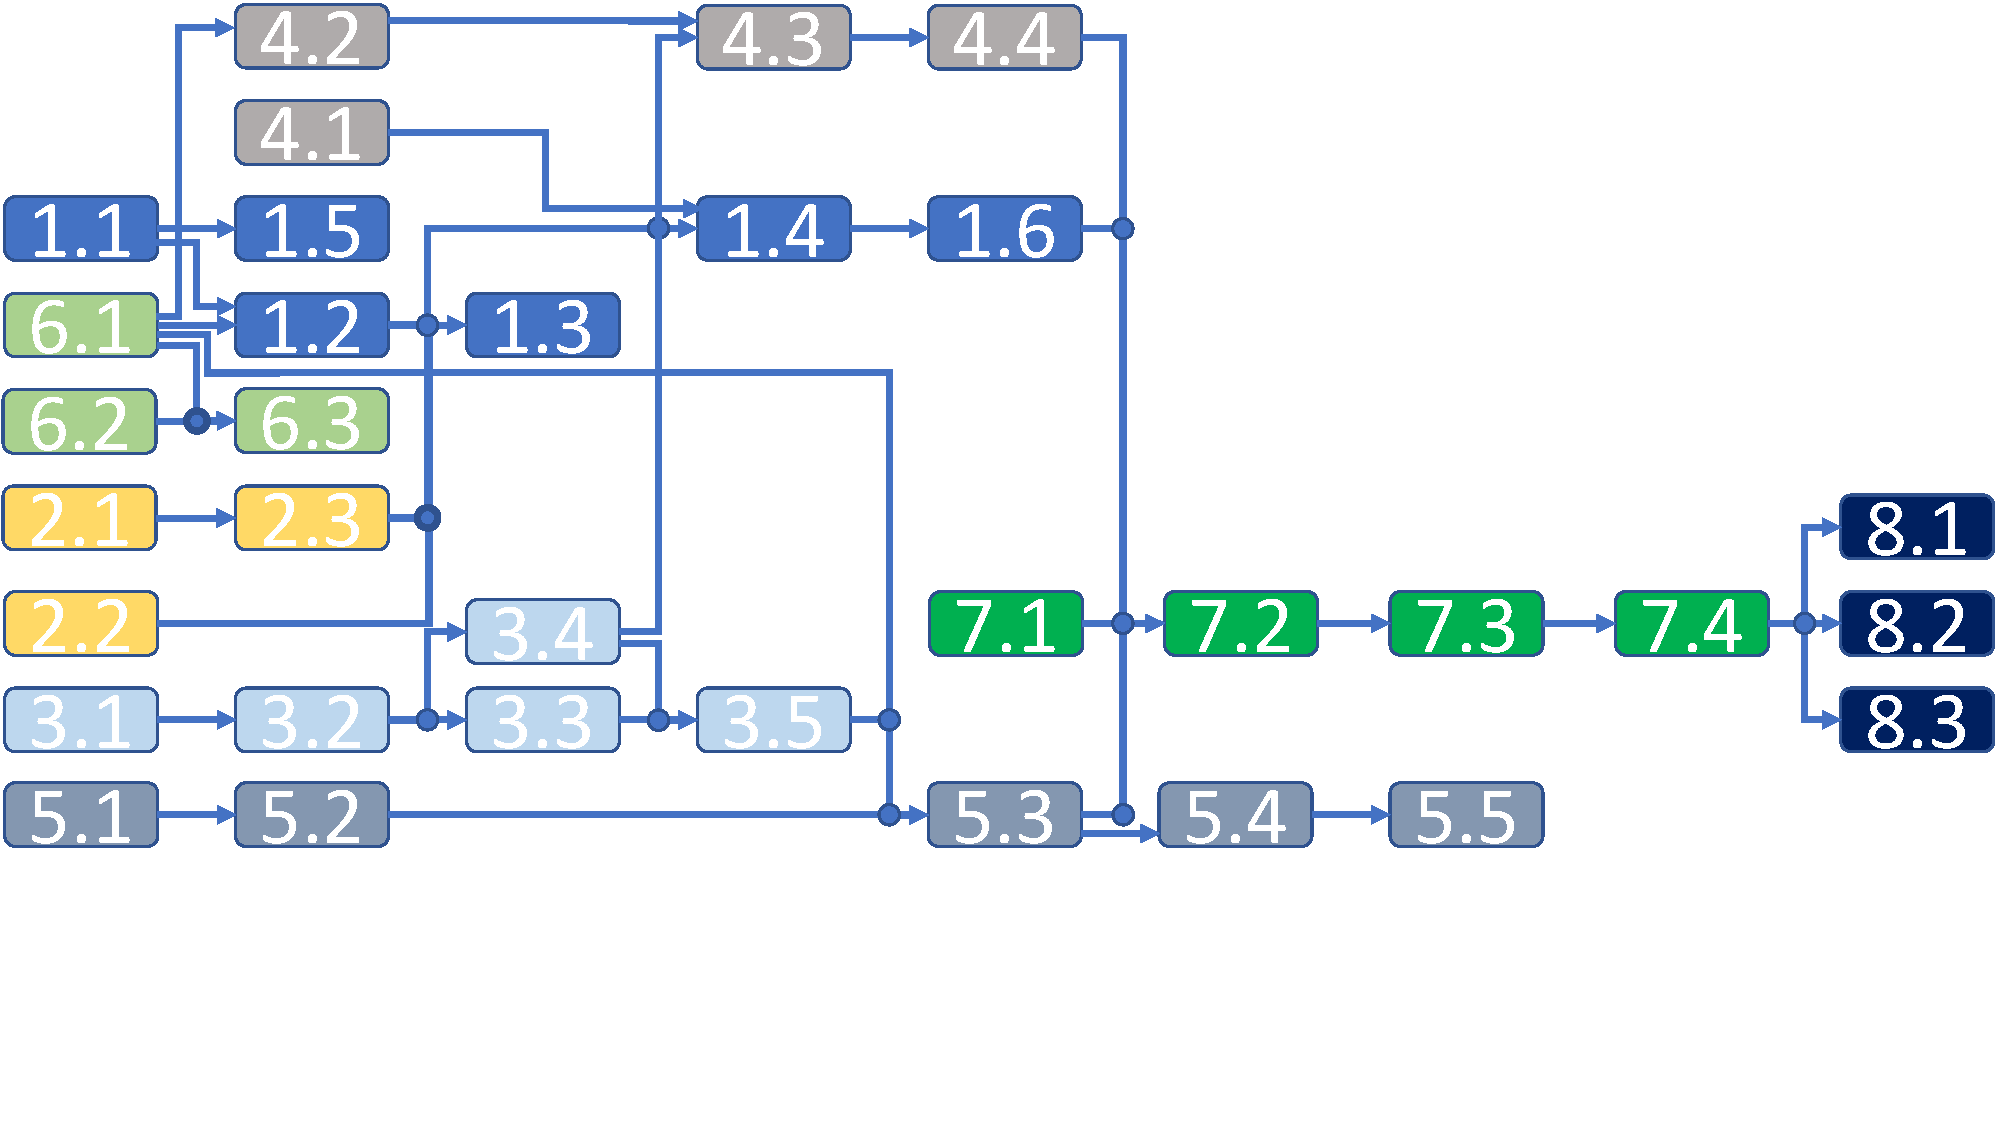
\includegraphics[width=.8\textwidth]{./Figuras/AoN.pdf}
	\caption{Diagrama en \textit{Activity on Node}}
	\label{fig:AoN}
\end{figure}

\section{11. Diagrama de Gantt}
\label{sec:gantt}


\begin{landscape}
	\begin{figure}[htpb]
		\centering
		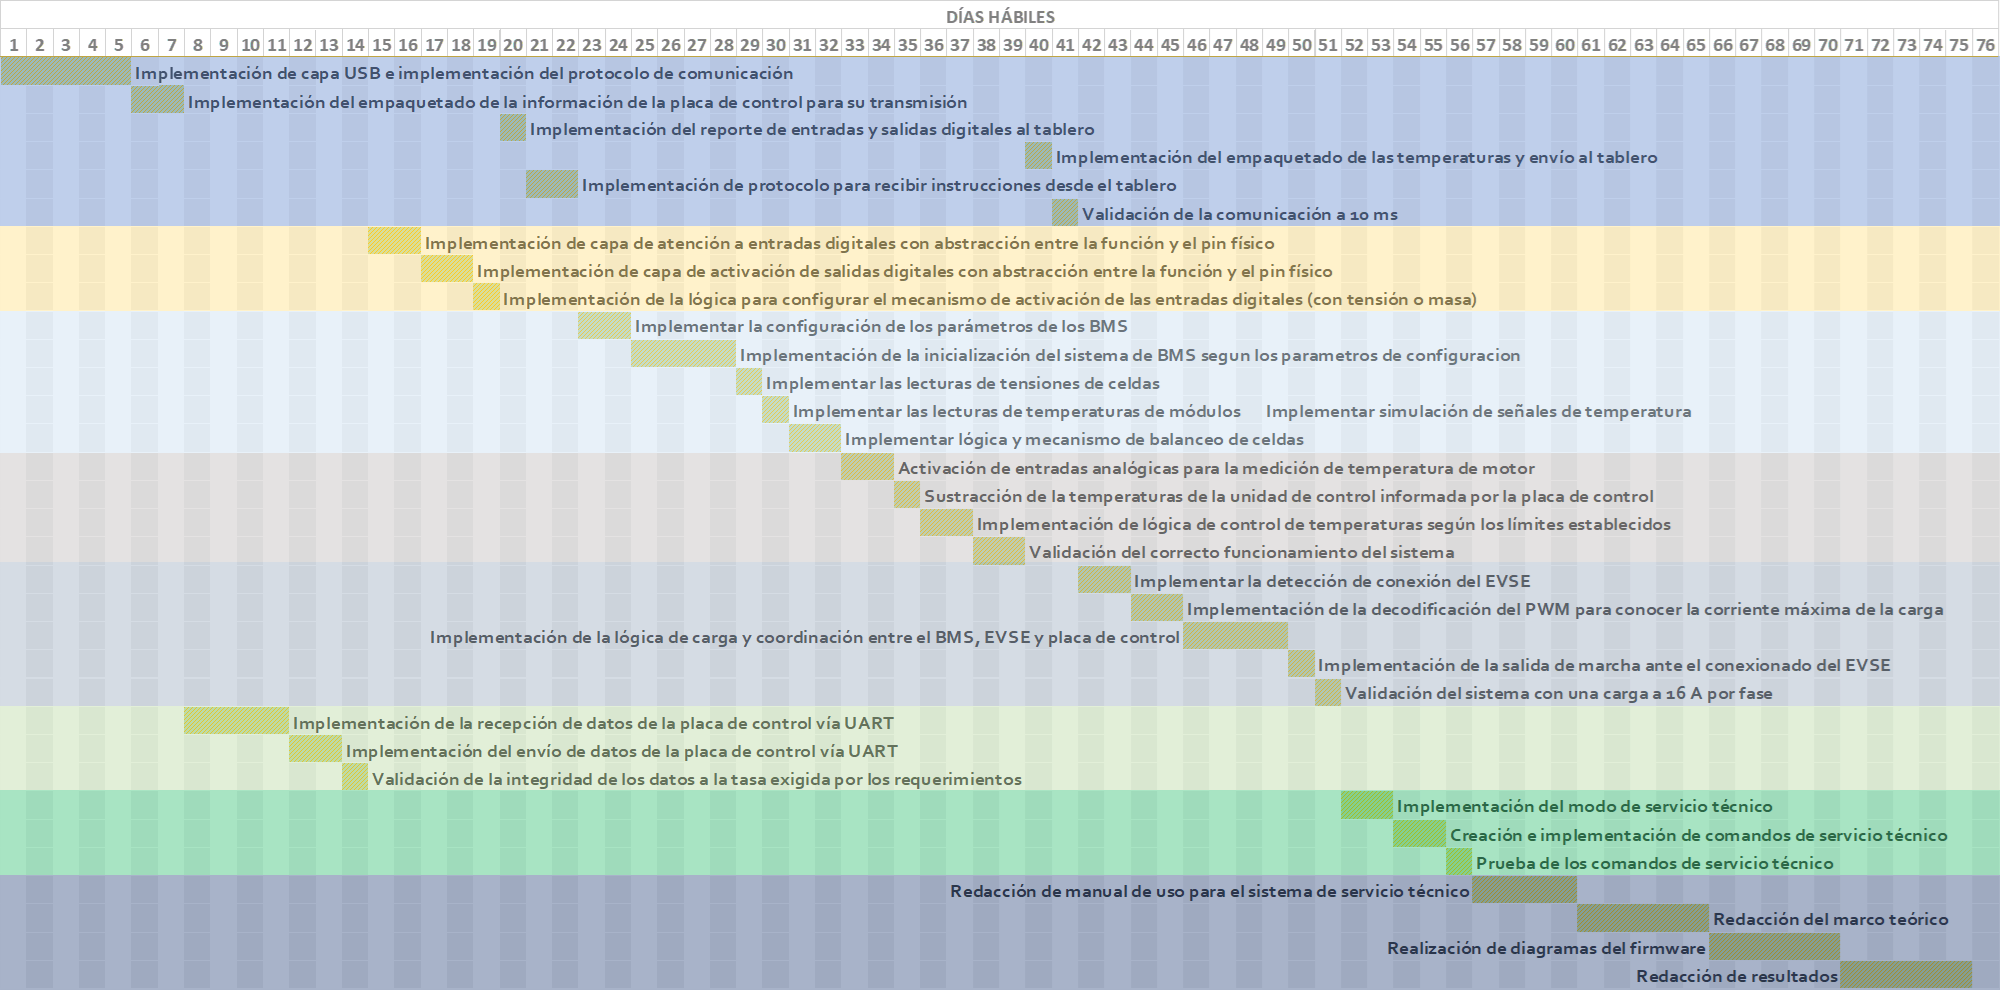
\includegraphics[height=.78\textheight]{./Figuras/Gantt.png}
		\caption{Diagrama de Gantt}
		\label{fig:diagGantt}
	\end{figure}

\end{landscape}



\section{12. Presupuesto detallado del proyecto}
\label{sec:presupuesto}

\begin{table}[htpb]
	\centering
	\begin{tabularx}{\linewidth}{@{}|X|c|r|r|@{}}
		\hline
		\rowcolor[HTML]{C0C0C0}
		\multicolumn{4}{|c|}{\cellcolor[HTML]{C0C0C0}COSTOS DIRECTOS}   \\ \hline
		\rowcolor[HTML]{C0C0C0}
		Descripción                                                 &
		\multicolumn{1}{c|}{\cellcolor[HTML]{C0C0C0}Cantidad}       &
		\multicolumn{1}{c|}{\cellcolor[HTML]{C0C0C0}Valor unitario} &
		\multicolumn{1}{c|}{\cellcolor[HTML]{C0C0C0}Valor total}        \\ \hline
		Placa de comunicaciones                                     &
		\multicolumn{1}{c|}{2}                                      &
		\multicolumn{1}{c|}{\$ 10.000}                              &
		\multicolumn{1}{c|}{\$ 20.000}                                  \\ \hline
		Placa de control                                            &
		\multicolumn{1}{c|}{2}                                      &
		\multicolumn{1}{c|}{\$ 15.000}                              &
		\multicolumn{1}{c|}{\$ 30.000}                                  \\ \hline
		EVSE                                                        &
		\multicolumn{1}{c|}{1}                                      &
		\multicolumn{1}{c|}{\$ 60.000}                              &
		\multicolumn{1}{c|}{\$ 60.000}                                  \\ \hline
		Modulo de baterías con BMS                                  &
		\multicolumn{1}{c|}{4}                                      &
		\multicolumn{1}{c|}{\$410.400}                              &
		\multicolumn{1}{c|}{\$1.641.640}                                \\ \hline
		Honorarios de desarrollador                                 &
		\multicolumn{1}{c|}{600}                                    &
		\multicolumn{1}{c|}{\$ 1.500}                               &
		\multicolumn{1}{c|}{\$ 900.000}                                 \\ \hline
		\multicolumn{3}{|c|}{SUBTOTAL}                              &
		\multicolumn{1}{c|}{\$ 2.651.640}                               \\ \hline
		\rowcolor[HTML]{C0C0C0}
		\multicolumn{4}{|c|}{\cellcolor[HTML]{C0C0C0}COSTOS INDIRECTOS} \\ \hline
		\rowcolor[HTML]{C0C0C0}
		Descripción                                                 &
		\multicolumn{1}{c|}{\cellcolor[HTML]{C0C0C0}Cantidad}       &
		\multicolumn{1}{c|}{\cellcolor[HTML]{C0C0C0}Valor unitario} &
		\multicolumn{1}{c|}{\cellcolor[HTML]{C0C0C0}Valor total}        \\ \hline
		\multicolumn{1}{|l|}{30\% de los costos directos}           &
		\multicolumn{1}{c|}{1}                                      &
		\multicolumn{1}{c|}{\$ 795.492}                             &
		\multicolumn{1}{c|}{\$ 795.492}                                 \\ \hline
		\multicolumn{3}{|c|}{SUBTOTAL}                              &
		\multicolumn{1}{c|}{\$ 294.300}                                 \\ \hline
		\rowcolor[HTML]{C0C0C0}
		\multicolumn{3}{|c|}{TOTAL}                                 &
		\multicolumn{1}{c|}{\$ 3.447.132}                               \\ \hline
	\end{tabularx}%
\end{table}


\section{13. Gestión de riesgos}
\label{sec:riesgos}

a) Identificación de los riesgos y estimación de sus consecuencias:

Riesgo 1: demora en la llegada de componentes del exterior.
\begin{itemize}
	\item Severidad (S): 8

	      La demora en la llegada de componentes del exterior, cuando son necesarios, detiene completamente el avance del proyecto.
	\item Probabilidad de ocurrencia (O): 9

	      Las demora de recursos del exterior es muy recurrente en Argentina.
\end{itemize}

Riesgo 2: el vínculo con la empresa se termine antes de lo establecido.
\begin{itemize}
	\item Severidad (S): 10.

	      No será posible realizar el proyecto.
	\item Ocurrencia (O): 2.

	      El vínculo actual con \clientename\hspace{1px}  es poco probable que finalice debido a que actualmente el autor trabaja en relación de dependencia para él.
\end{itemize}

Riesgo 3: accidentes graves en las verificaciones del proyecto debido a los riesgos asociados a la alta tensión.
\begin{itemize}
	\item Severidad (S): 10.

	      El Tren Motor utiliza tensiones mayores a 300 V. Esto puede causar daños graves y poner en riesgo el avance del proyecto.
	\item Ocurrencia (O): 5.

	      La constante manipulación de las placas con altas tensiones aumenta el riesgo de que se produzcan accidentes.
\end{itemize}

Riesgo 4: cancelación del proyecto del tren motor por decisión de la empresa.
\begin{itemize}
	\item Severidad (S): 10.

	      La cancelación del proyecto del tren motor torna innecesario el desarrollo de este proyecto.
	\item Ocurrencia (O): 2.

	      La tecnología actualmente es muy demandada desde el área comercial y no se presentan amenazas evidentes sobre la continuidad del proyecto.
\end{itemize}

Riesgo 5: subestimación de tiempos en tareas de la línea crítica.
\begin{itemize}
	\item Severidad (S): 6.

	      Este error en la planificación indefectiblemente atrasa todo el plan.

	\item Ocurrencia (O): 7.

	      El poco conocimiento sobre la complejidad del problema a resolver aumenta significativamente las probabilidades de error en la estimación de tiempos.
\end{itemize}
b) Tabla de gestión de riesgos:      (El RPN se calcula como RPN=SxO)
\begin{table}[htpb]
	\centering
	\begin{tabularx}{\linewidth}{@{}|X|c|c|c|c|c|c|@{}}
		\hline
		\rowcolor[HTML]{C0C0C0}
		Riesgo & S  & O & RPN & S* & O* & RPN* \\ \hline
		1      & 8  & 9 & 72  & 8  & 3  & 24   \\ \hline
		2      & 10 & 2 & 20  &    &    &      \\ \hline
		3      & 10 & 5 & 50  & 10 & 1  & 10   \\ \hline
		4      & 10 & 2 & 20  &    &    &      \\ \hline
		5      & 6  & 7 & 42  &    &    &      \\ \hline
	\end{tabularx}%
\end{table}

Criterio adoptado:
se tomarán medidas de mitigación en los riesgos cuyos números de RPN sean mayores a 45

Nota: los valores marcados con (*) en la tabla corresponden luego de haber aplicado la mitigación.

c) Plan de mitigación de los riesgos que originalmente excedían el RPN máximo establecido:

Riesgo 1: aprovechando que la lista de componentes está definida, se realizará el pedido con anticipación para asegurar un período de tiempo extenso desde que se piden los elementos al exterior hasta que se los necesite.

- Severidad (S): 8

La severidad no varía.

- Probabilidad de ocurrencia (O): 3

La anticipación reduce significativamente la probabilidad de que ocurra.

Riesgo 3: se utilizará serigrafía en la placa para indicar las regiones de alta tensión, se utilizará las protecciones y aislaciones necesarias para reducir la probabilidad de shock eléctrico.

- Severidad (S): 8

La severidad no varía.

- Probabilidad de ocurrencia (O): 2

Las medidas de seguridad y protocolización reduce significativamente la probabilidad de que ocurra.


\section{14. Gestión de la calidad}
\label{sec:calidad}

\begin{enumerate}
	\item Interfaces
	      \begin{enumerate}
		      \item El sistema debe poder comunicarse con el tablero con protocolo USB.

		            Verificación: en la base de datos generada por el tablero se visualiza que los datos cargados son los esperados luego de una carga y el uso en marcha del equipo.

		            Validación: el usuario visualiza la información del tablero correctamente.

		      \item El sistema debe poseer un botón de encendido

		            Verificación: el botón de encendido enciende el equipo cuando se presiona y apaga el equipo al mantenerse presionado por medio segundo.

		            Validación: el usuario puede encender y apagar el equipo.
		      \item El sistema debe poder actuar sobre los periféricos de refrigeración.

		            Verificación: la refrigeración se enciende y apaga cuando se alcanzan las temperaturas establecidas.

		            Validación: el usuario usa el equipo y las temperaturas se mantienen constantemente dentro de limites seguros.

		      \item El sistema debe responder a las señales digitales de los pulsadores y switches del vehículo. El tiempo de respuesta debe ser instantáneo para la percepción del usuario final (menor a 100 ms).

		            Verificación: se observa en la base de datos de la tablet que el estado de todas las entradas digitales son conmutadas al estimularlas con los pulsadores/switches.

		            Validación: el usuario usa las funcionalidades de los pulsadores y switches sin percibir demoras en la respuesta.
		      \item El sistema debe comunicarse con el BMS.

		            Verificación: se verifican que las tensiones y temperaturas reportadas por el BMS son las medidas con instrumentos de medición patrón.

		            Validación: el usuario no reporta fallas debido a errores en el BMS.

		      \item El sistema debe comunicarse con la placa de control. Esta comunicación debe ser redundante y robusta.

		            Verificación: se verifica que la placa de control responde a las ordenes de la placa de comunicaciones y la información recibida por la placa de control es la esperada durante una carga y una marcha.

		            Validación: el usuario siempre puede visualizar datos en el tablero que genera la placa de control (ej: temperatura de la unidad de control).
		      \item El sistema debe comunicarse con el EVSE.

		            Verificación: se puede completar un ciclo de carga.

		            Validación: el usuario puede cargar el vehículo sin inconvenientes.

	      \end{enumerate}
	\item Requerimientos funcionales
	      \begin{enumerate}
		      \item Comunicación con el tablero.
		            \begin{enumerate}
			            \item La taza de actualización de datos debe ser de 10 ms.

			                  Verificación: se verifica contando en el software del tablero que esa taza de datos se cumple.

			                  Validación: el usuario puede visualizar los datos en el tablero de forma continua.

			            \item Se debe transmitir al tablero toda la información reportada por la placa de control.

			                  Verificación: se verifica en la base de datos del tablero que la información de la placa de control se encuentra incorrupta.

			                  Validación: el servicio técnico puede ver toda la información del control cuando lo desea.

			            \item El estado de las entradas y salidas digitales debe ser reportado al tablero.

			                  Verificación: se verifica en la base de datos del tablero que el estado de las entradas y salidas digitales se encuentra correcto.

			                  Validación: el usuario puede visualizar el estado de las entradas y salidas digitales que manipula.
			            \item Las temperaturas de la unidad de control, batería y motor deben ser reportadas al tablero.

			                  Verificación: se verifica en la base de datos del tablero que las temperaturas de la unidad de control, batería y motor se encuentran correctas.

			                  Validación: el usuario puede visualizar las temperaturas de la unidad de control, batería y motor en el tablero.
			            \item El sistema puede ser configurado mediante el usuario a través del tablero.

			                  Verificación: se verifica que la placa de comunicaciones responde a los comandos de configuración.

			                  Validación: el usuario puede configurar el sistema.
		            \end{enumerate}
		      \item Entradas digitales
		            \begin{enumerate}
			            \item El sistema debe poder recibir señales digitales de los pulsadores y switches del vehículo.

			                  Verificación: se verifica que el sistema responde ante los estímulos de las señales digitales existentes

			                  Validación: el usuario puede puede utilizar las funcionalidades de los pulsadores y switches.
			            \item Las señales deben ser remapeables por cada vehículo, es decir, disociar el pin físico de la funcionalidad específica.

			                  Verificación: se verifica que las señales digitales se pueden remapear intercambiando las funcionalidades de los botones en un mismo \textit{set up}.

			                  Validación: los distintos vehículos tienen las funcionalidades acordes a sus necesidades y tableros.
			            \item La activación de las entradas digitales (con tensión o masa) deben ser configurables fuera del tiempo de compilación por personal de la empresa.

			                  Verificación: utilizando un switch se cambia la configuración de las entradas digitales y se verifica que cambia el comportamiento de las mismas. Responde por masa o tensión según la configuración seteada.

			                  Validación: los vehículos pueden ser configurados para responder por masa o tensión fácilmente.
		            \end{enumerate}
		      \item BMS
		            \begin{enumerate}
			            \item El sistema debe conocer el estado de todas las celdas.

			                  Verificación: se miden las tensiones de las celdas y se verifica que el sistema reporta las mismas tensiones en la base de datos.

			                  Validación: el equipo de servicio técnico puede visualizar las tensiones de las celdas en el tablero en modo servicio técnico.
			            \item El sistema debe conocer las temperaturas en el interior de todos los módulos de batería.

			                  Verificación: se miden las temperaturas de los módulos de batería y se verifica que el sistema reporta las mismas temperaturas en la base de datos.

			                  Validación: el equipo de servicio técnico puede visualizar las temperaturas de los módulos de batería en el tablero en modo servicio técnico. Además, el usuario puede ver cual es la temperatura máxima medida en la batería desde el tablero.
			            \item El sistema debe ser capaz de mantener las baterías balanceadas. Un máximo de 50 mV entre celdas.

			                  Verificación: se miden las tensiones de las celdas luego de un ciclo de carga y se verifica que no están desbalanceadas.

			                  Validación: el usuario puede verificar que las baterías están balanceadas durante el ciclo de vida del vehículo.
			            \item El sistema debe ser capaz de conectarse a distintas configuraciones de baterías según los parámetros del vehículo. Cada vehículo posee distinta cantidad de módulos y distintos modelos de módulos.

			                  Verificación: es posible conectarse a cualquiera de las 3 configuraciones de baterías existentes sin re-compilar el firmware.

			                  Validación: en producción el se puede instalar el tren motor con cualquier configuración de batería sin complicaciones.
		            \end{enumerate}
		      \item Control de temperaturas
		            \begin{enumerate}
			            \item El sistema debe conocer la temperatura de la unidad de control.

			                  Verificación: se miden las temperaturas de la unidad de control y se verifica que el sistema reporta las mismas temperaturas en la base de datos.

			                  Validación: el equipo de servicio técnico puede visualizar las temperaturas de los componentes la unidad de control en el tablero en modo servicio técnico. Además, el usuario puede ver cual es la temperatura de la unidad de control desde el tablero (un promedio de los componentes).
			            \item El sistema debe conocer la temperatura de la batería.

			                  Verificación: se miden las temperaturas de la batería y se verifica que el sistema reporta las mismas temperaturas en la base de datos.

			                  Validación: el equipo de servicio técnico puede visualizar las temperaturas de los módulos de batería en el tablero en modo servicio técnico. Además, el usuario puede ver cual es la temperatura máxima medida en la batería desde el tablero.
			            \item El sistema debe conocer la temperatura del motor.

			                  Verificación: se mide las temperatura del motor y se verifica que el sistema reporta las mismas temperaturas en la base de datos.

			                  Validación: el usuario puede ver cual es la temperatura máxima medida en el motor desde el tablero.

			            \item El sistema debe accionar los actuadores de refrigeración cuando la temperatura de algún componente exceda el 60\% de la temperatura de falla.

			                  Verificación: se verifica que los actuadores de refrigeración se activan cuando la temperatura de algún componente exceda el 60\% de la temperatura de falla. Los sensores se pueden calentar mediante una pistola de calor.

			                  Validación: el usuario utilizar el vehículo y este siempre está dentro de los límites de temperaturas de funcionamiento.

			            \item Las bombas de circulación de líquido deben accionarse siempre que el vehículo se encuentre en marcha o carga.

			                  Verificación: se verifica que las bombas de circulación de liquido se activan cuando el vehículo se encuentre en marcha o carga.

			                  Validación: las temperaturas de los componentes del vehículo se mantienen homogéneas durante la carga y marcha.

		            \end{enumerate}
		      \item Carga con EVSE
		            \begin{enumerate}
			            \item El sistema debe poder conectarse con un EVSE Mennekes.

			                  Verificación: al conectar un EVSE Mennekes se detecta la conexión por parte del sistema.

			                  Validación: el usuario confirma la conexión del EVSE Mennekes mediante un indicador visual (Led).
			            \item El sistema debe interpretar el limite de corriente que informa el EVSE para configurar el valor de la corriente de carga.

			                  Verificación: se verifica que el sistema carga a la corriente límite de la hoja de datos del equipo.

			                  Validación: el usuario puede cargar el vehículo y no reporta problemas por exceder la corriente limite.

			            \item El sistema debe conocer la temperatura del EVSE.

			                  Verificación: se miden las temperaturas del EVSE y se verifica que el sistema reporta las mismas temperaturas en la base de datos.

			                  Validación: el usuario conoce la temperatura del EVSE.

			            \item El sistema debe disparar la orden de carga a la placa de control cuando el EVSE esté conectado y listo para cargar.

			                  Verificación: se verifica que el sistema dispara la orden de carga a la placa de control cuando el EVSE esté conectado y listo para cargar.

			                  Validación: el usuario puede cargar el vehículo utilizando el EVSE, no reporta intentos de carga espontáneos o inesperados.

			            \item La placa de comunicaciones debe sacar al vehículo de marcha si detecta la conexión de un EVSE.

			                  Verificación: se verifica que la placa de comunicaciones saca al vehículo de marcha cuando detecta la conexión de un EVSE.

			                  Validación: el usuario no puede marchar el vehículo con el EVSE conectado al vehículo.
		            \end{enumerate}
		      \item Comunicación con placa de control
		            \begin{enumerate}
			            \item La placa de comunicaciones debe indicar a la placa de control el estado objetivo (marcha, carga o reposo).

			                  Verificación: se verifica con un analizador lógico que las ordenes se envían correctamente por la UART.

			                  Validación: las transiciones a marcha, carga y reposo suceden de la forma que pretende el usuario al utilizar el vehículo.

			            \item La placa de comunicaciones debe indicar a la placa de control la dirección de avance (Directa o Reversa).

			                  Verificación: se verifica con un analizador lógico que las ordenes se envían correctamente por la UART.

			                  Validación: el usuario puede utilizar el vehículo para ir en directa o reversa.

			            \item La placa de comunicaciones debe informar la tensión máxima y mínima de las celdas a la placa de control.

			                  Verificación: se verifica con un analizador lógico que se envía el dato adecuado a la placa de control.

			                  Validación: el tren motor sale del estado de marcha si una celda esta en una tensión muy baja (2.9 V).

			            \item La placa de comunicaciones debe ser capaz de recibir datos de la placa de control cada 10 ms.

			                  Verificación: se envían datos por la UART cada 10 ms hacia la placa de comunicaciones y se verifica que puede atenderlas sin comprometer las otras funcionalidades.

			                  Validación: el usuario puede utilizar el vehículo sin problemas con esta tasa de comunicación. Además, puede ver de forma continua los datos generados en la placa de control (visibles para el usuario).
		            \end{enumerate}
	      \end{enumerate}
	\item Requerimientos de robustez
	      \begin{enumerate}
		      \item El sistema debe ser capaz de mantener sus comunicaciones en condiciones ruidosas (aceleraciones fuertes o cargas rápidas).

		            Verificación: se verifica que el sistema no se ralentiza en condiciones de ruido confirmando la integridad de todos los datos de la base de datos ante aceleraciones o ciclos de carga.

		            Validación: el usuario ve con fluidez el tablero en todo momento al utilizar el vehículo.
	      \end{enumerate}
	\item Requerimientos de testing
	      \begin{enumerate}
		      \item El sistema debe ser poseer un modo de servicio técnico.

		            Verificación: se verifica que se puede acceder al modo de servicio técnico desde una PC mediante una conexión USB.

		            Validación: el servicio técnico puede conectarse a la placa mediante la interfaz de servicio técnico.

		      \item El modo de servicio técnico debe permitir probar los actuadores del sistema de forma independiente.

		            Verificación: se verifica que los actuadores del sistema responden correctamente a los comandos de servicio técnico.

		            Validación: se pueden diagnosticar los problemas de los actuadores del sistema o confirmar su correcto funcionamiento.
		      \item El modo de servicio técnico debe ser vía PC mediante el mismo USB del tablero.

		            Verificación: se verifica que el modo de servicio técnico puede conectarse a la placa mediante la interfaz de servicio técnico.

		            Validación: el personal de servicio técnico puede utilizar el modo de servicio técnico para diagnosticar los problemas de la placa desde su PC.
		      \item El modo de servicio técnico debe permitir la configuración de los parámetros del sistema.

		            Verificación: se verifica que los parámetros del sistema se pueden configurar desde el modo de servicio técnico cambiándolos y luego consultando su valor.

		            Validación: en producción se puede configurar los parámetros del sistema sin inconvenientes.


	      \end{enumerate}
\end{enumerate}
\section{15. Procesos de cierre}
\label{sec:cierre}

\begin{itemize}
	\item Análisis de correspondencia con el Plan de Proyecto original.
	      \begin{itemize}
		      \item Responsable: \authorname\hspace{1px}.
		      \item Se analizará cuales fueron los motivos que desviaron a las tareas retrasadas del plan original.
	      \end{itemize}
	\item Identificación de las técnicas y procedimientos útiles e inútiles que se emplearon, y los problemas que surgieron y cómo se solucionaron.
	      \begin{itemize}
		      \item Responsable: \authorname\hspace{1px}.
		      \item Se generará documentación durante el avance del proyecto sobre las técnicas y herramientas recurridas. Al finalizar se realizará un compendio con todas las herramientas que resultaron de mayor utilidad para el desarrollo del proyecto.
	      \end{itemize}
	\item Acto de agradecimiento a todos los interesados.
	      \begin{itemize}
		      \item Responsable: \authorname\hspace{1px}.
		      \item Se realizará un acto por la plataforma Meet para agradecer a todos los que hicieron posible el desarrollo del proyecto: colaboradores, profesores de la maestría y el equipo de trabajo.
	      \end{itemize}
\end{itemize}



\end{document}
